\section{Benchmarks}

\label{sec:benchmarks}

All benchmarks were conducted on Zoo testnet (chain ID 200201) using the following hardware:

\begin{itemize}
    \item \textbf{Validator nodes}: 21 nodes, each with AMD EPYC 7763 (64 cores), 512GB RAM, NVIDIA A100 80GB
    \item \textbf{Load generators}: 10 nodes generating transactions via JSON-RPC
    \item \textbf{Network}: 10 Gbps interconnect, geographically co-located
\end{itemize}

\subsection{Workload Categories}

We benchmark five workload categories representative of Zoo Network usage:

\begin{enumerate}
    \item \textbf{Token Transfers}: ERC-20 \texttt{transfer()} calls (21,000 gas each)
    \item \textbf{AMM Swaps}: Zoo DEX precompile swaps via LP-9012 (85,000 gas each)
    \item \textbf{AI Inference}: Precompile calls for model inference (500,000 gas each)
    \item \textbf{FHE Operations}: TFHE/CKKS operations via 0x0700 precompile (65,000--420,000 gas)
    \item \textbf{Complex DeFi}: Multi-hop swaps with flash loans (350,000 gas each)
\end{enumerate}

\subsection{Raw Execution Throughput}

\begin{table}[t]
\centering
\begin{tabular}{lccccc}
\toprule
\textbf{Workload} & \textbf{Gas/TX} & \textbf{TXs/Block} & \textbf{Exec (ms)} & \textbf{TPS (exec)} & \textbf{TPS (final)} \\
\midrule
Token Transfer & 21K & 47,619 & 1.0 & 47.6M & 4.76M \\
AMM Swap & 85K & 11,764 & 2.8 & 4.2M & 1.17M \\
AI Inference & 500K & 2,000 & 8.5 & 235K & 200K \\
FHE (ckksMul) & 65K & 15,384 & 4.2 & 3.66M & 1.54M \\
Complex DeFi & 350K & 2,857 & 6.1 & 468K & 285K \\
\bottomrule
\end{tabular}
\caption{Raw execution throughput. ``TPS (exec)'' is GPU execution only; ``TPS (final)'' includes 10ms Quasar finality.}
\label{tab:throughput}
\end{table}

\subsection{Latency Distribution}

\begin{figure}[t]
\centering
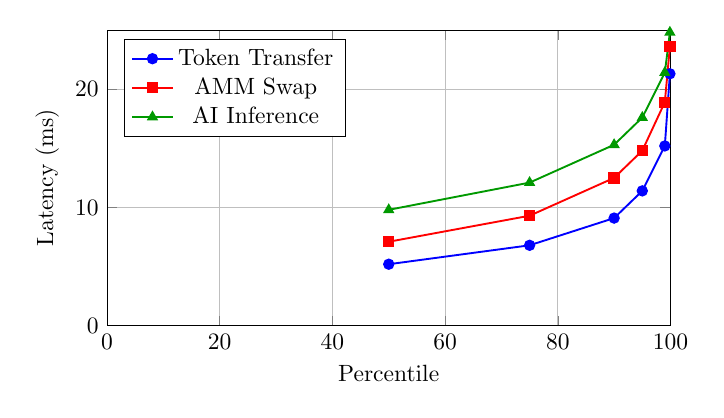
\begin{tikzpicture}[scale=0.85]
    \begin{axis}[
        xlabel={Percentile},
        ylabel={Latency (ms)},
        xmin=0, xmax=100,
        ymin=0, ymax=25,
        legend pos=north west,
        grid=major,
        width=10cm,
        height=6cm
    ]
    \addplot[blue, thick, mark=*] coordinates {
        (50, 5.2) (75, 6.8) (90, 9.1) (95, 11.4) (99, 15.2) (99.9, 21.3)
    };
    \addlegendentry{Token Transfer}

    \addplot[red, thick, mark=square*] coordinates {
        (50, 7.1) (75, 9.3) (90, 12.5) (95, 14.8) (99, 18.9) (99.9, 23.6)
    };
    \addlegendentry{AMM Swap}

    \addplot[green!60!black, thick, mark=triangle*] coordinates {
        (50, 9.8) (75, 12.1) (90, 15.3) (95, 17.6) (99, 21.4) (99.9, 24.8)
    };
    \addlegendentry{AI Inference}
    \end{axis}
\end{tikzpicture}
\caption{End-to-end latency distribution (submission to finality) for three workload types on Zoo testnet.}
\label{fig:latency}
\end{figure}

Median end-to-end latency (transaction submission to Quasar finality) is 5.2ms for token transfers, 7.1ms for AMM swaps, and 9.8ms for AI inference calls. The p99 latency remains under 22ms for all workload types.

\subsection{GPU Utilization}

\begin{table}[t]
\centering
\begin{tabular}{lccc}
\toprule
\textbf{Workload} & \textbf{GPU Util (\%)} & \textbf{GPU Mem (GB)} & \textbf{Shader Occupancy} \\
\midrule
Token Transfer & 34\% & 8.2 & 82\% \\
AMM Swap & 52\% & 14.6 & 76\% \\
AI Inference & 89\% & 42.1 & 94\% \\
FHE Operations & 78\% & 31.4 & 88\% \\
Complex DeFi & 61\% & 18.9 & 71\% \\
\bottomrule
\end{tabular}
\caption{GPU resource utilization by workload type on NVIDIA A100 80GB.}
\label{tab:gpu}
\end{table}

AI inference workloads achieve 89\% GPU utilization, demonstrating that the GPU EVM efficiently exploits hardware parallelism for compute-heavy operations. Simple token transfers underutilize the GPU (34\%) because they are memory-bound rather than compute-bound.

